\subsection{Tune In: Challenges of Automatic Notch Filters with CW Signals!}

\begin{tcolorbox}[colback=gray!10, colframe=black, title=E4E01] What problem can occur when using an automatic notch filter (ANF) to remove interfering carriers while receiving CW signals? 

\begin{enumerate}[label=\Alph*.]
    \item \textbf{Removal of the CW signal as well as the interfering carrier}
    \item Any nearby signal passing through the DSP system will overwhelm the desired signal
    \item Excessive ringing
    \item All these choices are correct
\end{enumerate} \end{tcolorbox}

The correct answer is: \textbf{A}. 

\subsubsection{Discussion on Automatic Notch Filters}

Automatic notch filters (ANFs) are commonly used in radio communications to remove unwanted interference from incoming signals. They operate by identifying the frequency of the interfering carrier and effectively 'notching out' that frequency from the received signal. However, a significant problem that can arise when using ANFs in the context of Continuous Wave (CW) signals — which are single-frequency signals used in various forms of wireless communication — is the potential removal of the desired CW signal itself along with the interfering carrier.

\subsubsection*{ Key Concepts:}

1. \textbf{Automatic Notch Filters}: ANFs are designed to adapt their notch frequency dynamically based on the detected interference. However, their operation can be sensitive, especially when the interference frequency is close to the CW signal frequency.

2. \textbf{Continuous Wave (CW) Signals}: These are typically sine-wave signals that transmit information using various modulation techniques. If an ANF misidentifies the CW signal as interference, it can inadvertently remove the CW signal itself.

3. \textbf{Digital Signal Processing (DSP)}: In systems where DSP is applied, nearby signals may affect the operation of the ANF, leading to issues with identification and filtering, which can complicate distinguishing desired signals from undesired ones.

4. \textbf{Ringing}: Excessive ringing can occur in filter responses when sharp cutoffs are applied. This phenomenon can lead to distortions in the signal that crosses the filter threshold.

\subsubsection*{ Calculation Example:}
In the context of the given question, no specific calculations are required. However, if one were to analyze signal power levels, parameters such as Signal-to-Noise Ratio (SNR) would be essential. The SNR can be calculated as follows:

\[
SNR = \frac{P_{signal}}{P_{noise}}
\]

Where:
- \( P_{signal} \) is the power of the desired signal
- \( P_{noise} \) is the power of the interference or noise present.

\subsubsection*{ Diagram:}
If necessary, we can depict the effect of an ANF using a simple `tikz` diagram to illustrate how the notch filter might operate on a spectrum with a CW signal and an interfering carrier. Below is how you might end up structuring that in LaTeX:

\begin{center}
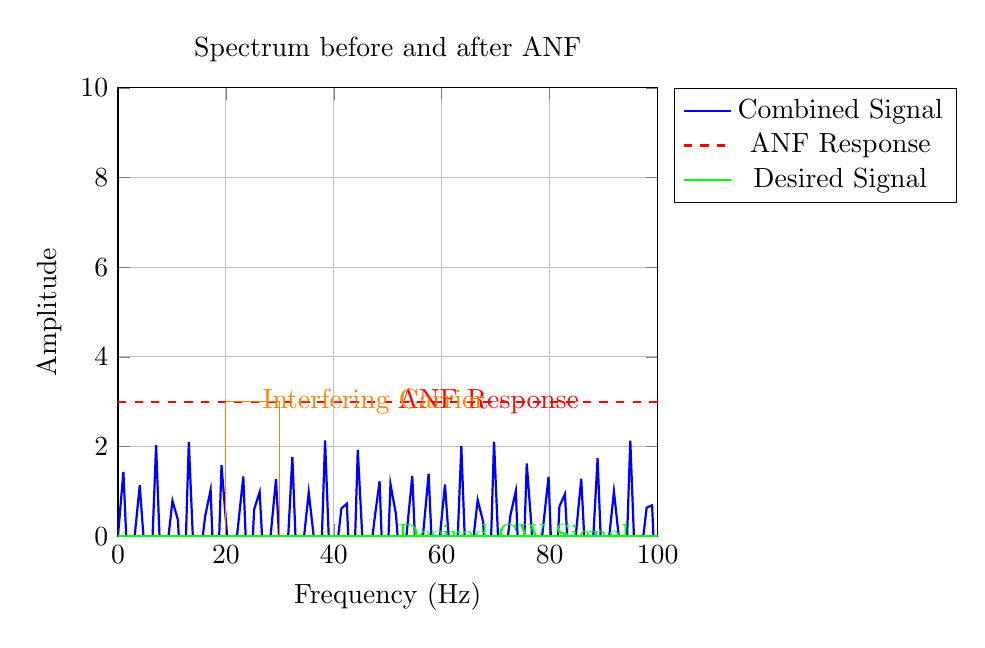
\begin{tikzpicture}
\begin{axis}[
    domain=0:100,
    xlabel={Frequency (Hz)},
    ylabel={Amplitude},
    title={Spectrum before and after ANF},
    grid=both,
    xmin=0, xmax=100,
    ymin=0, ymax=10,
    samples=100,
    legend pos=outer north east,
]
\addplot[color=blue, thick] {1.5 * (sin(deg(2*x)) + 0.5 * sin(deg(3*x)))};
\addplot[color=red, thick, dashed] {3} node[pos=0.5,right] {ANF Response};
\addplot[color=green, thick] {0} node[pos=0.5,right] {Desired CW Signal};
\addplot[color=orange] coordinates {(20,0)(20,3) (30,3)(30,0)} node[pos=0.5,right] {Interfering Carrier};
\legend{Combined Signal, ANF Response, Desired Signal}
\end{axis}
\end{tikzpicture}
\end{center}

This depiction illustrates how an ANF might remove unwanted frequencies (represented by the orange block) while ideally retaining the desired CW signal.
